\documentclass[tikz,border=10pt]{standalone}
\usetikzlibrary{arrows.meta, positioning, calc}

\begin{document}
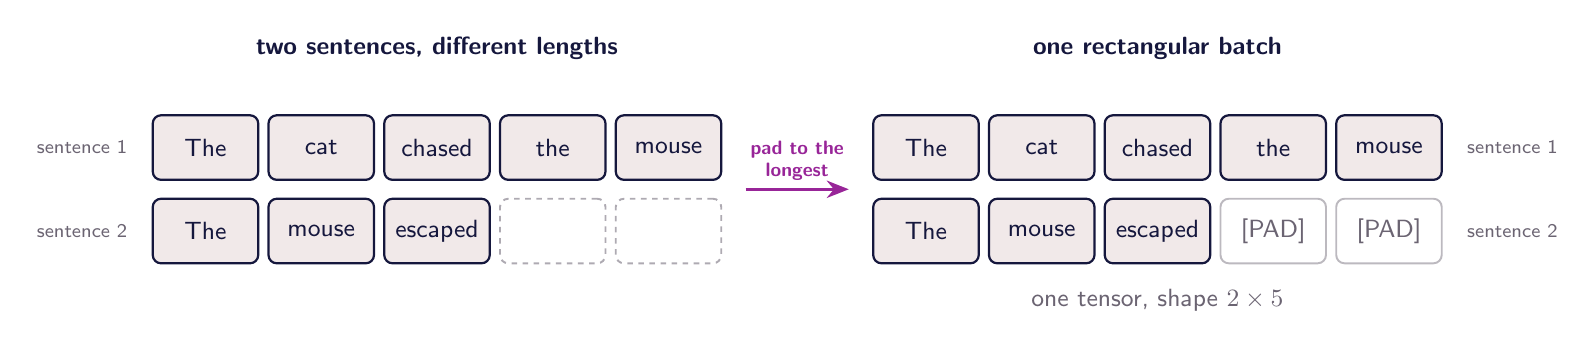
\begin{tikzpicture}[
    every node/.style={font=\sffamily},
]

% ---------------------------------------------------------------- colours
\definecolor{c1}{HTML}{15173D}   % the words, the boxes
\definecolor{c2}{HTML}{982598}   % the operative step (the padding)
\definecolor{c3}{HTML}{E491C9}
\definecolor{c4}{HTML}{F1E9E9}
\definecolor{axiscolor}{HTML}{333333}
\definecolor{labelcolor}{HTML}{6B6472}

% ================================================================
% Geometry, decided before any TikZ was written.
%
%   word box 1.34 x 0.82, pitch 1.47  ->  horizontal gap 0.13
%   two rows, y = 0 (sentence 1) and y = -1.06 (sentence 2)
%   vertical gap between rows 0.24: tight enough to read as a block
%
%   LEFT panel  columns x = 0, 1.47, 2.94, 4.41, 5.88   (spans -0.67 .. 6.55)
%   RIGHT panel columns are the same shifted by \dx = 9.15
%                        x = 9.15 ... 15.03             (spans  8.48 .. 15.70)
%   gutter 6.55 .. 8.48, 1.93 wide, completely empty of boxes
%
%   arrow: (6.86, -0.53) -> (8.17, -0.53), the vertical midline of the block
%   its two-line label sits above it, centred in the gutter at x = 7.515, so it
%   cannot touch either panel
%
%   row labels once, on the far left, right-anchored at x = -0.95: both panels
%   sit on the same two rows, so one pair of labels names both
%
%   titles at y = 0.95 (0.55 above the box tops), annotation under the right
%   panel at y = -1.62 (0.17 below the row-2 box bottoms)
%
%   bounding box roughly x in [-2.5, 17.7], y in [-2.1, 1.3]: wide and short
% ================================================================

\def\pitch{1.47}
\def\dx{9.15}
\def\rowa{0}
\def\rowb{-1.06}

\tikzset{
    wordbox/.style={
        draw=c1, line width=0.8pt, fill=c4,
        rounded corners=3pt,
        minimum width=1.34cm, minimum height=0.82cm,
        inner sep=0pt,
    },
    emptyslot/.style={
        draw=labelcolor, line width=0.7pt, dashed, dash pattern=on 2pt off 2pt,
        opacity=0.55,
        rounded corners=3pt,
        minimum width=1.34cm, minimum height=0.82cm,
        inner sep=0pt,
    },
    padbox/.style={
        draw=labelcolor, line width=0.7pt, draw opacity=0.45,
        rounded corners=3pt,
        minimum width=1.34cm, minimum height=0.82cm,
        inner sep=0pt,
    },
    word/.style={font=\sffamily\small, text=c1},
    rowlab/.style={font=\sffamily\scriptsize, text=labelcolor, anchor=east},
    title/.style={font=\sffamily\small\bfseries, text=c1, anchor=south},
    note/.style={font=\sffamily\small, text=labelcolor, anchor=north},
    arr/.style={draw=c2, line width=1.1pt,
        -{Stealth[length=2.8mm, width=2.2mm]}},
}

% ================================================================ LEFT panel
\node[title] at (2.94, 1.00) {two sentences, different lengths};

% sentence 1, five words
\foreach \i/\w in {0/The, 1/cat, 2/chased, 3/the, 4/mouse} {
    \pgfmathsetmacro{\x}{\i*\pitch}
    \node[wordbox] at (\x, \rowa) {};
    \node[word]    at (\x, \rowa) {\w};
}

% sentence 2, three words and two slots that simply are not there
\foreach \i/\w in {0/The, 1/mouse, 2/escaped} {
    \pgfmathsetmacro{\x}{\i*\pitch}
    \node[wordbox] at (\x, \rowb) {};
    \node[word]    at (\x, \rowb) {\w};
}
\foreach \i in {3,4} {
    \pgfmathsetmacro{\x}{\i*\pitch}
    \node[emptyslot] at (\x, \rowb) {};
}

% ================================================================ row labels
\node[rowlab] at (-0.87, \rowa) {sentence 1};
\node[rowlab] at (-0.87, \rowb) {sentence 2};

% ================================================================ the arrow
\draw[arr] (6.86, -0.53) -- (8.17, -0.53);
\node[font=\sffamily\scriptsize\bfseries, text=c2, anchor=south,
      align=center, inner sep=0pt]
    at (7.515, -0.42) {pad to the\\longest};

% ================================================================ RIGHT panel
\node[title] at (2.94+\dx, 1.00) {one rectangular batch};

\foreach \i/\w in {0/The, 1/cat, 2/chased, 3/the, 4/mouse} {
    \pgfmathsetmacro{\x}{\i*\pitch+\dx}
    \node[wordbox] at (\x, \rowa) {};
    \node[word]    at (\x, \rowa) {\w};
}
\foreach \i/\w in {0/The, 1/mouse, 2/escaped} {
    \pgfmathsetmacro{\x}{\i*\pitch+\dx}
    \node[wordbox] at (\x, \rowb) {};
    \node[word]    at (\x, \rowb) {\w};
}
\foreach \i in {3,4} {
    \pgfmathsetmacro{\x}{\i*\pitch+\dx}
    \node[padbox] at (\x, \rowb) {};
    \node[font=\sffamily\small, text=labelcolor] at (\x, \rowb) {[PAD]};
}

% the right panel repeats the row labels, on its own right-hand side:
% the gutter is spoken for by the arrow
\node[rowlab, anchor=west] at (15.90, \rowa) {sentence 1};
\node[rowlab, anchor=west] at (15.90, \rowb) {sentence 2};

\node[note] at (2.94+\dx, -1.68) {one tensor, shape $2 \times 5$};

\end{tikzpicture}
\end{document}
